%%%%%%%%%%%%%%%%%%%%%%%%%%%%%%%%%%%%%%%%%%%%%%%%%%%%%%%%%%
\begin{frame}[fragile]
\frametitle{A Very Simple Application Example}
%%%%%%%%%%%%%%%%%%%%%%%%%%%%%%%%%%%%%%%%%%%%%%%%%%%%%%%%%%


\begin{lstlisting}
val sc = new SparkContext("spark://...", "MyJob", home, jars) 

val file = sc.textFile("hdfs://...") // This is an RDD

val errors = file.filter(_.contains("ERROR")) // This is an RDD

errors.cache()

errors.count() // This is an action
\end{lstlisting}

\end{frame}

%%%%%%%%%%%%%%%%%%%%%%%%%%%%%%%%%%%%%%%%%%%%%%%%%%%%%%%%%%
\begin{frame}
\frametitle{Spark Applications: The Big Picture}
%%%%%%%%%%%%%%%%%%%%%%%%%%%%%%%%%%%%%%%%%%%%%%%%%%%%%%%%%%
\begin{itemize}
	\item There are two ways to manipulate data in Spark
	\begin{itemize}
		\item Use the interactive shell, \textit{i.e.,} the REPL
		\item Write standalone applications, \textit{i.e.,} driver programs
	\end{itemize}
\end{itemize}

	\begin{figure}[h]
	  \centering
	  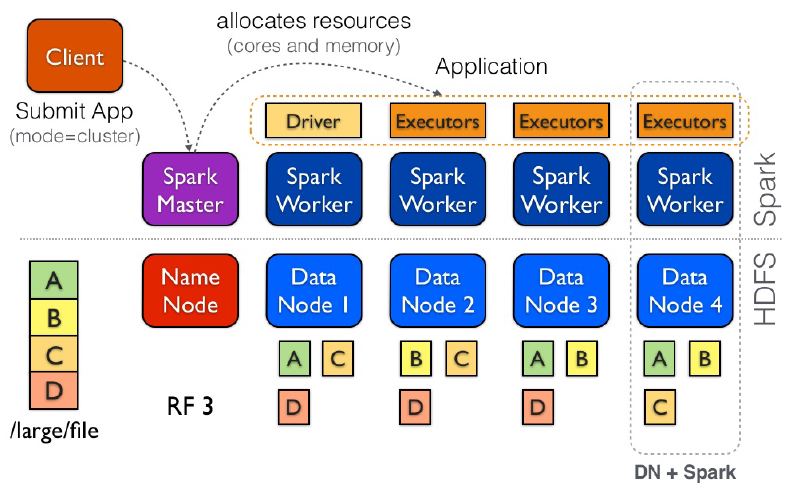
\includegraphics[scale=0.33]{./Figures/spark_app_overview}
	  \label{fig:spark_app_overview}
	\end{figure}
\end{frame}

%%%%%%%%%%%%%%%%%%%%%%%%%%%%%%%%%%%%%%%%%%%%%%%%%%%%%%%%%%
\frame {\frametitle{Spark Components: details}
%%%%%%%%%%%%%%%%%%%%%%%%%%%%%%%%%%%%%%%%%%%%%%%%%%%%%%%%%%
\begin{figure}[h]
  \centering
  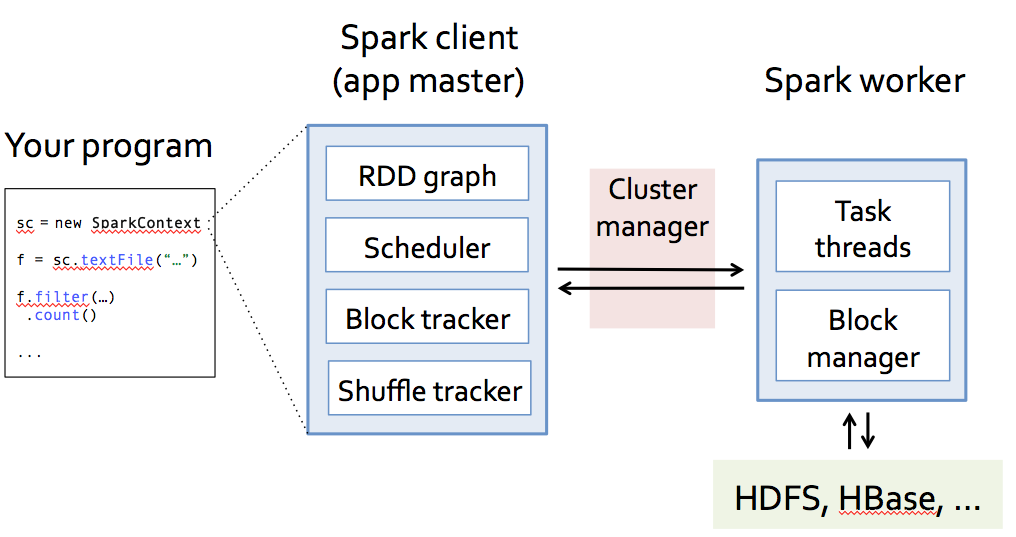
\includegraphics[scale=0.33]{./Figures/spark_components}
  \label{fig:spark_components_details}
\end{figure}
}


%%%%%%%%%%%%%%%%%%%%%%%%%%%%%%%%%%%%%%%%%%%%%%%%%%%%%%%%%%
\frame {\frametitle{The RDD graph: dataset vs. partition views}
%%%%%%%%%%%%%%%%%%%%%%%%%%%%%%%%%%%%%%%%%%%%%%%%%%%%%%%%%%
% missing: what is an rdd? difference between RDD and partition?

\begin{columns}[c]
	\column{.5\textwidth}
		
			\begin{figure}[h]
			  \centering
			  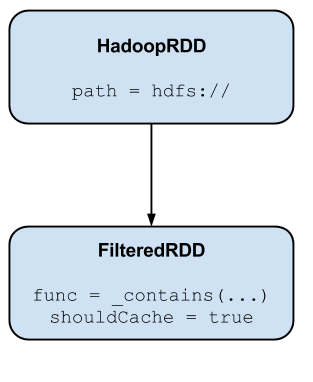
\includegraphics[scale=0.25]{./Figures/spark_rdd}
			  \label{fig:spark_components}
			\end{figure}
	
	\column{.5\textwidth}
		
			\begin{figure}[h]
			  \centering
			  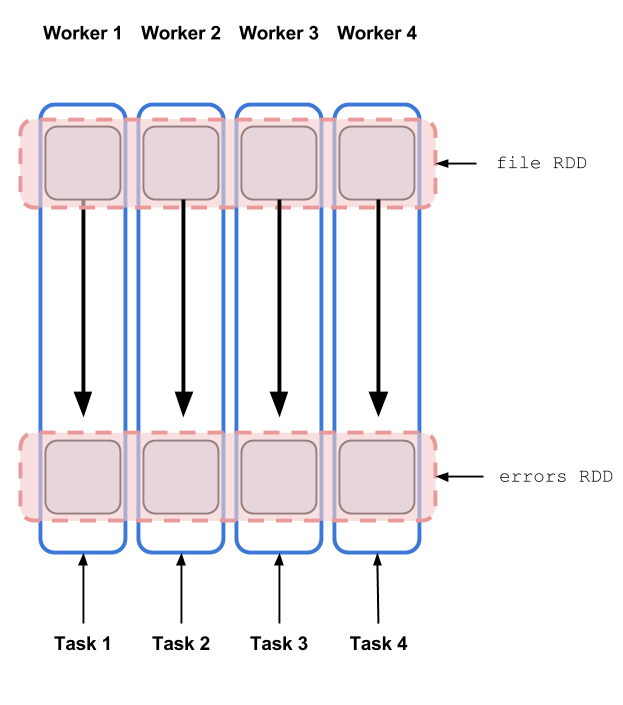
\includegraphics[scale=0.25]{./Figures/spark_partition}
			  \label{fig:spark_components}
			\end{figure}

\end{columns}
}

% %%%%%%%%%%%%%%%%%%%%%%%%%%%%%%%%%%%%%%%%%%%%%%%%%%%%%%%%%%
\frame {\frametitle{Data Locality}
% %%%%%%%%%%%%%%%%%%%%%%%%%%%%%%%%%%%%%%%%%%%%%%%%%%%%%%%%%%
\begin{itemize}
	\item {\bf Data locality principle}
	\begin{itemize}
		\item Same as for Hadoop MapReduce
		\item Avoid network I/O, workers should manage local data
	\end{itemize}

	\vspace{20pt}

	\item {\bf Data locality and caching}
	\begin{itemize}
		\item First run: data not in cache, so use HadoopRDD's locality prefs (from HDFS)
		\item Second run: FilteredRDD is in cache, so use its locations
		\item If something falls out of cache, go back to HDFS
	\end{itemize}
\end{itemize}
}



%%%%%%%%%%%%%%%%%%%%%%%%%%%%%%%%%%%%%%%%%%%%%%%%%%%%%%%%%%
\frame {\frametitle{Lifetime of a Job in Spark}
%%%%%%%%%%%%%%%%%%%%%%%%%%%%%%%%%%%%%%%%%%%%%%%%%%%%%%%%%%

\begin{columns}[t, onlytextwidth]
	\begin{column}[T]{.2\textwidth}
		\begin{center}
			{ \tiny \bf RDD Objects}
		\end{center}
		\begin{figure}[h]
			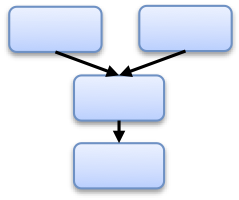
\includegraphics[scale=0.5]{./Figures/RDD_objects}
		\end{figure}

		\begin{colorblock}{blue}{lightblue}{ }
			{\tiny \texttt{
				rdd1.join(rdd2)\\
				\hspace{12pt} .groupBy(...)\\
				\hspace{12pt} .filter(...)\\
				}
			}
		\end{colorblock}

		\vspace{10pt}

		\begin{colorblock}{blue}{lightblue}{ }
			{\tiny \bf Build the operator DAG}
		\end{colorblock}
	\end{column}

	\begin{column}[T]{.2\textwidth}
		\begin{center}
			{ \tiny \bf DAG Scheduler}
		\end{center}			
		\begin{figure}[h]
			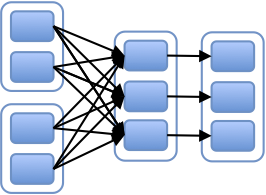
\includegraphics[scale=0.5]{./Figures/DAG_scheduler}
		\end{figure}

		\vspace{10pt}

		\begin{colorblock}{blue}{lightblue}{ }
			{\tiny \bf Split the DAG into \emph{stages} of \emph{tasks}}
		\end{colorblock}

		\vspace{10pt}

		\begin{colorblock}{blue}{lightblue}{ }
			{\tiny \bf Submit each stage and its tasks as ready}
		\end{colorblock}			
	\end{column}

	\begin{column}[T]{.2\textwidth}
		\begin{center}
			{ \tiny \bf Task Scheduler}
		\end{center}			

		\vspace{-20pt}

		\begin{figure}[h]
			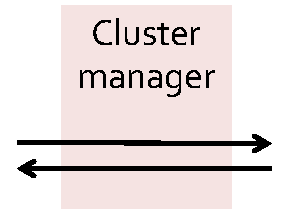
\includegraphics[scale=0.5]{./Figures/Task_scheduler}
		\end{figure}

		\vspace{10pt}

		\begin{colorblock}{blue}{lightblue}{ }
			{\tiny \bf Launch tasks via Master}
		\end{colorblock}

		\vspace{10pt}

		\begin{colorblock}{blue}{lightblue}{ }
			{\tiny \bf Retry failed and straggler tasks}
		\end{colorblock}			
	\end{column}

	\begin{column}[T]{.2\textwidth}
		\begin{center}
			{ \tiny \bf Worker}
		\end{center}			
		\begin{figure}[h]
			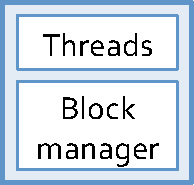
\includegraphics[scale=0.5]{./Figures/Worker}
		\end{figure}
		\vspace{10pt}

		\begin{colorblock}{blue}{lightblue}{ }
			{\tiny \bf Execute tasks}
		\end{colorblock}

		\vspace{10pt}

		\begin{colorblock}{blue}{lightblue}{ }
			{\tiny \bf Store and serve blocks}
		\end{colorblock}			
	\end{column}
\end{columns}
}

% %%%%%%%%%%%%%%%%%%%%%%%%%%%%%%%%%%%%%%%%%%%%%%%%%%%%%%%%%%
\frame {\frametitle{In Summary}
% %%%%%%%%%%%%%%%%%%%%%%%%%%%%%%%%%%%%%%%%%%%%%%%%%%%%%%%%%%
\begin{itemize}
	\item {\bf Our example Application}: a \textbf{jar} file
	\begin{itemize}
		\item Creates a \texttt{SparkContext}, which is the core component of the driver
		\item Creates an input RDD, from a file in HDFS
		\item Manipulates the input RDD by applying a \texttt{filter(f: T => Boolean)} transformation
		\item Invokes the action \texttt{count()} on the transformed RDD
	\end{itemize}

	\item {\bf The DAG Scheduler}
	\begin{itemize}
		\item Gets: RDDs, functions to run on each partition and a listener for results
		\item Builds \emph{Stages} of \emph{Tasks} objects (code + preferred location)
		\item Submits Tasks to the \textbf{Task Scheduler} as ready
		\item Resubmits failed \emph{Stages}
	\end{itemize}

	\item {\bf The Task Scheduler}
	\begin{itemize}
		\item Launches \emph{Tasks} on executors
		\item Relaunches failed \emph{Tasks}
		\item Reports to the DAG Scheduler
	\end{itemize}

\end{itemize}

}
